


\chapter{Introduction}

In this chapter I discuss firstly the broader context of research which relates to interactive annotation as it applies to this work. I discuss the topics in general, but also focus on applications to image processing with \gls{CNN}s. In section \ref{sec:closest} I then spend some time to compare and contrast the most specific research efforts most similar to this work.

\section{Research goals and contributions}

The central thesis to this dissertation is that annotation of data can be performed as a collaboration between human and machine learning algorithm. This by itself is not new idea, and is known as 'human in the loop' machine learning. Given the wide variety of visual recognition task, and thus different kinds of work-flow for annotation - I look to provide the best set of tools to empower the human annotator.

Specifically I look at two aspects where a machine learning algorithm assists a human annotator. The first and main focus is verification based annotation where a human annotator annotates a dataset by validating machine generated predictions.

The second focus is organising data and example selection - allowing an annotator to sort images, then find the best images to annotate first and then find mistakes or inconsistencies. 

A large part of crowd sourced annotation is having cross verification. I look at how a machine learning algorithm can help verify a dataset instead, to weed out errors by finding and showing inconsistencies in the provided data.

I explore the topic in a modern scenario using \gls{CNN}s, and aim to show the approach is very practical for annotation of a range of visual recognition datasets. I do this through developing tools for human in the loop image annotation and performing a series of experiments to answer questions and validate my ideas. I also demonstrate it's use on a series of real world image annotation tasks.


\subsection {Thesis summary and contributions}

This thesis is split into roughly two parts, firstly works which stand alone - and is presented first, chapter \ref{chap:focus} where I look at the effect of cropping and resolution on image classification, and \ref{chap:metric} where I experiment with a new method of metric learning for instance recognition, a kind of n-way siamese network. 

The rest of the thesis from \ref{chap:bootstrap} onward is devoted to the central topic of the thesis, namely human in the loop machine learning. In chapter \ref{chap:bootstrap} I discuss verification based annotation for segmentation data where images are annotated by drawing masks over areas of interest. I explore several angles for assisted image annotation, and conclude that the verification based bootstrapping process to be the most promising. Contrary to popular belief that \gls{CNN}s require much data and much training time. I demonstrate the opposite that using few images, and also very little training time a \gls{CNN} can be trained to a level to provide very real assistance to a human annotator. 

In chapters \ref{chap:object_detection} I describe  object detection \gls{CNN} model and look at properties useful for human in the loop annotation. I look at practical aspects of training, including training one class at a time, cyclical learning rates and experiment on several small scale (but real world) datasets. 


Chapter \ref{chap:object_detection} is devoted to the design and implementation of a human in the loop annotation system 

I also look at example selection methods, where I look at how an annotation tool can facilitate annotation workflows for different kinds of image data. I briefly explore methods of effectively reviewing existing annotations for consistency, and how unlabelled data can be more effectively sorted and processed.

I demonstrate the utility of the tool by annotating several new object detection datasets (and validate it on a few older ones),  and collaborate with others who use it to annotate datasets.



\subsection {Rapid prototyping}

Not only is it necessary to collect and annotate data - one of the primary questions asked when considering the use of machine learning is 'How many examples are necessary?'. To which the usual answer is to by experimental validation where part of the data is held back and used to test the effectiveness of training on the other part. In this work I don't change 



\section {Thesis structure}


\section {Background}

Crowd sourcing. Human in the loop. verification based annotation.

Uncertainty, active learning.

Related ideas are are those which aim to make more effective use of data available. This includes methods to enrich existing data such as semi-supervised learning and hard example mining \cite{Jin2018, Yu2018, Canevet2014}, as well as those aiming to accelerate the learning process by sampling the data in the right order, including curriculum learning and self paced learning.

Transfer learning attempts to accelerate learning on a new domain by using knowledge gained through learning on another (usually much larger and more general) domain. It has been shown that (especially for images with \gls{CNN}s) that models trained on these datasets can be re--purposed in a variety of useful ways.


\subsection {Crowd Sourcing}

The most common approach to annotating a dataset is crowd sourcing. Crowd sourcing enlists the services of many in order to provide 

Most large scale datasets are created with some form of crowd sourcing, notable examples ImageNet classification \cite{JiaDeng2009}, Coco object detection \cite{Lin2014} or Cityscapes street scenes \cite{Cordts2016} are all created with crowd sourcing. 

In order to get a lot of people to contribute there exist methods such as gamification, where the task is turned into a fun game  e.g. a game Quick Draw \cite{Ha2017}, or presenting the task as proof of humanness \cite{Goodfellow2013a}. Citizen science uses volunteers to perform tasks, for example to count penguins, identify species or identify planets \cite{Simpson2014, Masters2016}. Often the feeling of contributing to something meaningful, or the novelty of having your name as a contributor is enough to bring people to be involved.

If there exists no easy way to bring people to help for free, then use of labour markets such as \gls{AMT} are an option. These markets enable an employer to pay for mechanical tasks involving human intelligence. Many large scale datasets such as ImageNet \cite{Russakovsky2015} are built with \gls{AMT}. 


\subsection{Human in the loop}

Human in the loop machine learning encompasses a range of machine learning techniques which utilise human input in effective ways. Either by providing assistance to a human annotator with verification based annotation, or by having the annotator assist a learner which tries to make the most out of annotator time, such as active learning.

Machine learning datasets often contain a lot of so called ``easy'' examples. These examples often dominate both the annotation process where human time is spent needlessly annotating similar easy examples, and in the learning process where the learning algorithm spends much of it's computation time on examples which are already handled well. 


\subsection{Verification based annotation}

\begin{figure}[h]
  \centering
  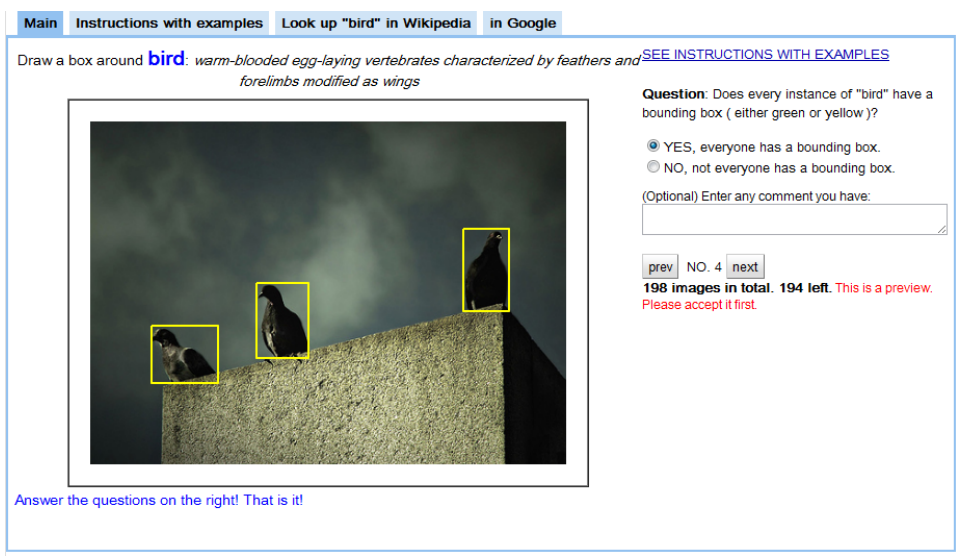
\includegraphics[width=1.0\linewidth]{introduction/crowdsourcing_annotation.jpg}
  \caption{Crowd sourcing image verification task in \cite{Su2012a}} 
  \label{fig:crowdsourcing}
\end{figure}

I coin the term verification based annotation, where machine annotations are checked and verified by a human annotator. Although the idea has played a central role in many previous works, it is not given an easily recognisable term to distinguish it for example from other kinds of Human in the Loop machine learning such as Active Learning (and is often put in the same basket). A selection of verification based methods, many of them discussed in detail below \cite{Yao2012, McNeill2011, Adhikaria2018, Castrejon2017, Papadopoulos2016, Russakovsky2015a}. 

Verification also plays a large part in ensuring consistency even between human annotators in crowd sourcing efforts, where the annotations of any one user cannot be fully trusted - users are tasked with cross verifying each others' annotations in many of these efforts. An example of a crowd sourcing task \cite{Su2012a} for verifying boxes is shown in figure \ref{fig:crowdsourcing}.

Weaker algorithms (machine learning or otherwise) can be used to generate proposals which can be then validated by an annotator. An example of this is in \cite{McNeill2011} where computer vision algorithms generate proposed counts of a penguin colony, and a human operator marks false negatives and false positives.

Human verification is fast, in \cite{Papadopoulos2016} reports a yes/no verification as taking 1.6 seconds on average. For a full annotation of an \gls{ILSVRC} image \cite {Su2012a} the time to draw a bounding box is reported at 26 seconds (42 seconds after quality control), but \cite{Papadopoulos2017} reports only 7 seconds per box using a more effective input method involving clicking extremities of objects rather than selecting corners. 

\begin{figure}[h]
  \centering
  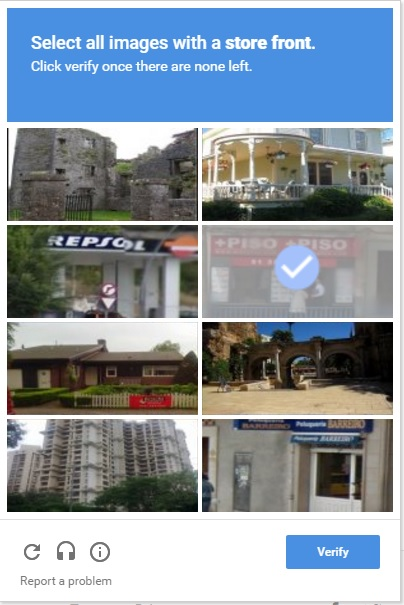
\includegraphics[width=0.5\linewidth]{introduction/recaptcha.jpg}
  \caption{reCAPTCHA dialog showing multi-image verification task}  
  \label{fig:captcha}
\end{figure}

The human ability to verify many examples at once has often be used, for example in recent tasks presented by the well known reCAPTCHA \cite{von2008recaptcha} a grid of images is presented asking a user to select all instances containing a particular object or type of scene, this is shown in figure \ref{fig:captcha}. To my knowledge there is no study confirming if visually validating multiple occurrences together is more efficient than validating single occurrences, but given it's wide use it seems that is likely the case. 

Previous studies on verification based annotation such as \cite{Papadopoulos2016} focuses on localisation for the ImageNet dataset which features typically few large object instances per image (due to it's origins as an image classification dataset), with smaller instances often in the background. On domains with many smaller objects such as in biological studies of animals, verifying many instances at once should be much more effective. 


\subsection{Example selection and active Learning} 

One prominent ``human in the loop'' method is active learning. Active learning revolves around picking the best set of examples for a human to annotate making most effective use of their time. Picking the best examples is often based around an uncertainty measure, where examples which a model is most uncertain about would often be the hard cases which are most useful for learning. 
 
While a \gls{CNN} used for classification provides some measure of uncertainty in it's output by way of it's softmax outputs, but this is usually not recommended and deemed unreliable. In \cite{Guo2017} it is shown that modern neural network architectures often systematically over estimate confidence, so it is important to find unbiased methods to estimate uncertainty.

\gls{CNN}s with accurate uncertainty measures are much in their infancy, especially for more complex tasks such as object detection. However recent research gone into more effectively quantifying uncertainty in \gls{CNN}s with tools such as Bayesian \gls{CNN}s \cite{Gal2017} and other methods of estimating uncertainty have arisen such as ensemble variation \cite{Beluch2018} or minibatch variation \cite{Chang2017}. 

Specific to object detection one recent approach is to measure the stability of predicted boxes when noise is added to inputs \cite{Kao2018}. Another idea is to measure consistency between bounding box proposals \cite{Kao2018, Brust2018, Le2018}. Current state of the art object detectors such as \gls{SSD} \cite{Liu2016a}, or \gls{RCNN} \cite{Wang2017} produce a multitude of box proposals - as such the variation can be measured.

Another measure used in active learning is expected change. An example of this is \cite{Vondrick2011} for video annotation, in which frames are selected for annotation which cause large expected change in the object track. Another example is \cite{Xu2017} where the expected change in an image's segmentation is used for the purpose of selecting which superpixels. 

Another related but distinct idea is making the best use of the examples available and in the best order. Curriculum learning and self paced learning \cite{Kumar2010} are research efforts devoted to this goal. Curriculum learning aims to learn from the most informative examples of a dataset in order to learn faster and more reliably, (a recent example is \cite{Katharopoulos2018}) self paced learning also attempts to have the learning algorithm also determine which examples are hard and easy as it progresses.


\subsection{Semi-supervised learning}

Semi-supervised methods are another active research area which aims to save on annotation time - commonly either a dataset with only a small portion of labels, or a dataset with labels but lacking localisation annotation. Enriching a dataset with localisation information is studied because of the availability of large scale image datasets with class labels, methods include using the internal activity of a \gls{CNN} to infer location of objects in an image \cite{Sivic2015}, or consensus forming methods such as \cite{Sangineto} which uses a self-paced learning method beginning with the most reliable examples first, or \cite{Cinbis2017} using multiple data folds to ensure consistency. The later is used to bootstrap the question answering verification method \cite{Papadopoulos2016}.

Hard negative and example mining are commonplace in object detection methods to enrich annotations provided. Hard negative mining is commonly used in training where negative examples are not explicitly annotated, yet are necessary to ensure balanced training. In \gls{SSD} \cite{Liu2016a} in each training image the highest confidence non matching  box proposals are taken as negative examples. An alternative (used in this work) is that of Focal Loss \cite{Lin2017} which samples negative examples densely from unmatched boxes and re-weights the loss function to deal with the large ratio of unmatched to matched boxes.


\subsection{Interactive machine learning}

Many human in the loop processes (those which use human refinement to train a learner) are technically a form of interactive machine learning, but more specifically interactive machine learning uses human inputs to make predictions or modify it's behaviour directly.

Interactive machine learning is often used for segmentation where it takes considerable effort to input a segmentation mask, much more than to draw a bounding box for example. Object selection for example the GrabCut algorithm \cite{Rother} can be used to find object masks with approximate user input, such as scribbles or bounding box selection. Such a tool can be used iteratively to create, then refine an annotation with the annotator observing the output and making changes to the inputs.  LabelMe \cite{Russell2007} interface provides a scribble based object mask creation tool in this mould. 

\begin{figure}[h]
  \centering
  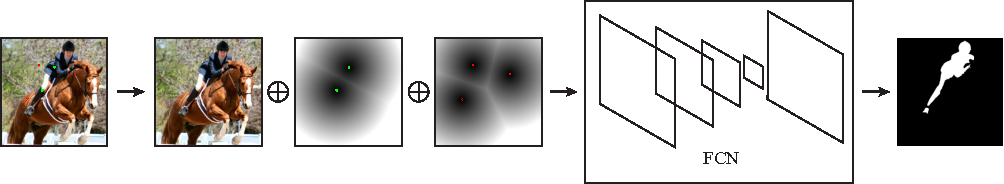
\includegraphics[width=1.0\linewidth]{introduction/object_selection.pdf}
  \caption{Object selection process from \cite{Xu2016b}, user input as clicks are turned into distance maps which are concatenated as input to a \gls{FCN} segmentation network}  
  \label{fig:object_selection}
\end{figure}

More recently, the same ideas have been applied using \gls{CNN}s where a model can be trained to predict an object mask based on user input, for example clicks \cite{Xu2016b, Boroujerdi2017}, bounding boxes \cite {Xu2017} or extreme points \cite{Maninis2017}. These methods train on datasets containing mask information (without caring about the classes given to the objects) and human input can be simulated based on the mask and bounding box annotations. An illustration of the process from \cite{Xu2016b} is shown in figure \ref{fig:object_selection}. Human input can also be used to refine an output for example in medical segmentation \cite{Wang2017}, or for image colourisation \cite{Zhang} where it's primary purpose is to provide a more intuitive editing tool.

A contrasting interactive approach is to have a model provide outputs designed to be easily editable, such as PolygonRNN \cite{Castrejon2017} which provides automatic object selection by bounding box, but provides outputs as a polygon rather than as a mask. The benefit of this approach is that a polygon can be edited more precisely and fed back into training directly.


\subsection {Transfer learning}

Transfer learning is the idea of taking knowledge gained from a base task, and applying it to another. The most prominent and widespread use of transfer learning is perhaps the use of fine tuning or feature extraction.  Where models trained on classification tasks (typically ImageNet \cite{JiaDeng2009}) are re-purposed for usually much smaller scale tasks in different ways. 

\gls{DECAF} \cite{Donahue2014} showed features extracted from the hidden layers of a \gls{CNN} were directly transferable to achieve the then state of the art on a number of image tasks, including classification and as a much stronger replacement for the hand crafted \gls{SURF} descriptor \cite{bay2006surf}.  Specifically they used AlexNet  \cite{Krizhevsky2012} trained on ImageNet \cite{JiaDeng2009}.

In \cite{Yosinski} it is shown that the transfer-ability of features depends on the distance between the base task to the target task, and that using a pre--trained network can even improve generalisation after fine tuning (as compared to training from scratch).

Fine tuning retrains a network for a new task, typically using a lower (or zero) learning rate for some parts in order to preserve the learned 

The use of pre-trained models is now commonplace in adapting \gls{CNN} to new domains, with repositories of state of the art models pre-trained on large datasets existing for most machine learning frameworks (for example the PyTorch \cite{Paszke2017} model zoo. 

It is becoming standard practice, models for other tasks - for example segmentation or object detection are usually based around a network (the so called backbone of a network) which has previously been trained on a classification task. Examples include the widely used \gls{FPN} network, \cite{Lin2017a} where a base network, for example a ResNet \cite{He} or a DenseNet \cite{Huang2016} backbone which operates from high resolution to low, is combined by a secondary path which operates from low resolution to high with shortcut connections between, combining a pattern seen before in the segmentation U--Net \cite{Ronneberger2015} architecture with pre-trained models.

The \gls{FPN} is now used as a base model in a variety of state of the art segmentation and object detection methods, and seems widely applicable to a variety of tasks by attaching different network ``heads'' specific to the task at hand (such as classification, regression etc.).




\section {Most similar projects to this work}
\label{sec:closest}

\subsection {Interactive Object Detection \cite{Yao2012}}
Interactive object detection \cite{Yao2012} describes a human in the loop interactive annotation system, where an incremental object detector (Hough forest) is trained as a user corrects annotations provided by the system. 

The user interface consists of the ability to delete incorrectly predicted instances (\gls{FP}) and to add new bounding boxes where the object detector failed to produce them (\gls{FN}). A user study was done and found that \gls{FN} were almost twice as expensive as \gls{FP} to correct. Though it is not mentioned the exact mechanism required from the user to implement these edits. It could be because the cost of drawing a box is faster than selecting one for deletion.


The work in this thesis has a similar focus in many aspects, notably using an object detection algorithm with a predict--refine--train loop. 

In contrast, an emphasis is placed on active learning and predicting the amount of time required for a user to correct the object predictions provided by the model, in this thesis the focus on enabling the user. 

Hough forests \cite{Gall2011} are used as an online learning method for the purposes of being fast to train and fast for inference. One disadvantage of hough forests is that when annotation mistakes are made then the decision trees which arise from those mistakes can not be reversed. 

In this thesis I focus on using \gls{CNN} based object detectors (particularly RetinaNet \cite{Lin2017} and \gls{FPN} \cite{Lin2017a}) for the same purpose, which benefit from recent developments in object detection and are in general much more capable object detectors. Compared to the hough forests described, training can be slower, but inference is much faster on a modern \gls{GPU} than the figures provided for the hough forest (13 seconds).



\subsection{Fluid Annotation \cite{Andriluka2018}}
\begin{figure}[h]
  \centering
  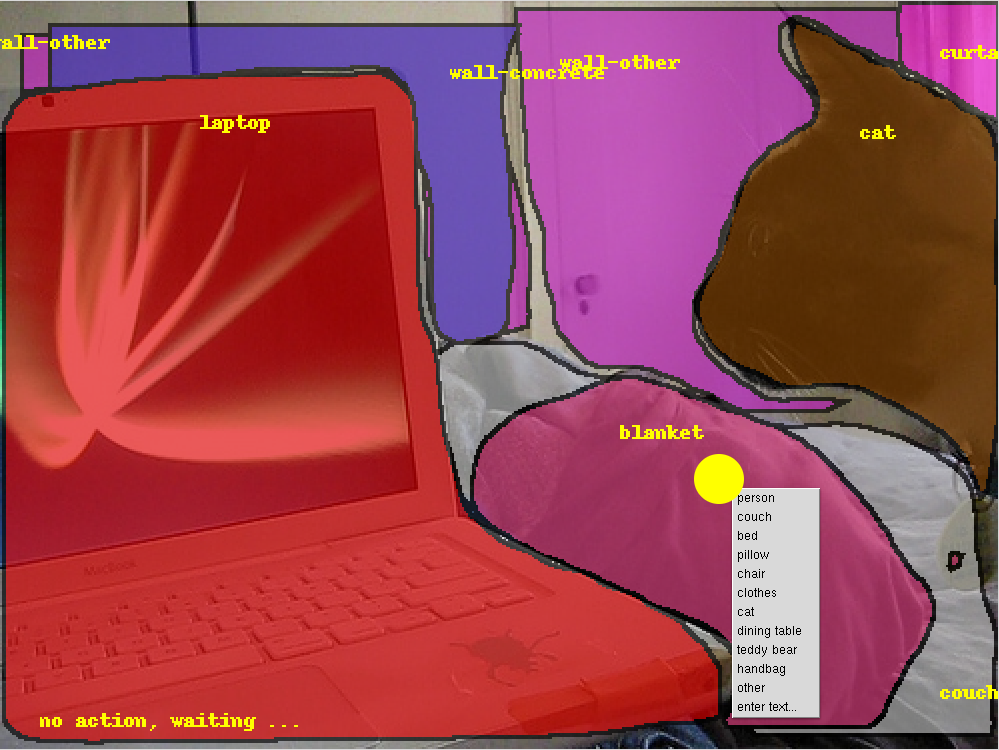
\includegraphics[width=1.0\linewidth]{introduction/fluid_annotation.png}
  \caption{User interface for Fluid Annotation \cite{Andriluka2018}}  
  \label{fig:fluid_annotation}
\end{figure}

Fluid annotation is an interactive human in the loop approach for instance segmentation. They point out three key points of their approach, the use of a strong neural network model, editing an entire image at once (as opposed to asking questions about each annotation one by one), and the approach to empower the annotator rather than employing clever methods to select examples (such as active learning). An example of the user interface is shown in figure \ref{fig:fluid_annotation}.

A key difference to my approaches is that I focus on annotating and experimentation with new domains, using transfer learning as a tool to enable online learning of the new domain. The strong neural network provides a power annotation aid, but limits you to annotate images in the same domain as that network (which is fine for many tasks).

\subsection{Faster Bounding Box Annotation for Object Detection in Indoor Scenes}

\begin{figure}[h]
  \centering
  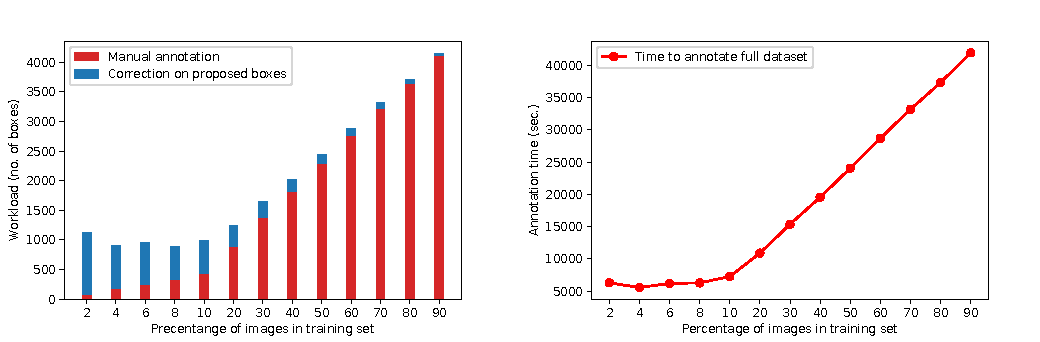
\includegraphics[width=1.0\linewidth]{introduction/adhikaria2018.pdf}
  \caption{Annotation time with different levels of manual annotation vs. assisted annotation. \cite{Adhikaria2018}}  
  \label{fig:adhikaria2018}
\end{figure}

In \cite{Adhikaria2018}, an object detection dataset is annotated in two parts, first a small split is fully manually annotated and used to train an initial model, then the remaining data is annotated by having the human annotator verify and refine model predictions. My approach is similar in many ways, the difference is that I focus on iterating annotation and training immediately with an incremental learning approach.

The advantage of splitting manual annotation and assisted annotation is is a simpler analysis of annotation effort. Figure \ref{fig:adhikaria2018} shows the relation between the number of manually annotated images and the time taken to annotate the rest of the images using assisted annotation.



\subsection {PolygonRNN \cite{Castrejon2017}}

\begin{figure}[h]
  \centering
  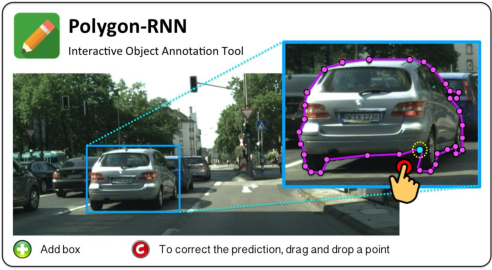
\includegraphics[width=1.0\linewidth]{introduction/polygon_rnn.pdf}
  \caption{The predict and refine process used in PolygonRNN \cite{Castrejon2017}}  
  \label{fig:polygon_rnn}
\end{figure}


Polygon-RNN \cite{Castrejon2017} uses a predict, refine, train approach in generating segmentation masks (as polygons), where a model is trained to segment generic objects then it can be fine tuned for a specific tasks where a user first provides a bounding box around an object, the model predicts a polygon and the refines the polygon and it is fed back for training. An illustration of this process is shown in figure \ref{fig:polygon_rnn} where user first selects a box around an instance, the model then predicts a sequence of points forming a polygon, the user then refines those points to better match the truth of the outline.

In this work I have a very similar goal with my work in chapter \ref{chap:bootstrap}, except instead of points I use masks. The advantage of points over masks is better edibility and potentially simpler outlines (PolygonRNN has some control in it's model over how fine the detail is between points). Editing with masks also has some advantages, it can provide discontinuous regions and operate without instance recognition. In chapter \ref{chap:annotation} this work focuses on object detection annotation for the whole scene, where PolygonRNN operates on each detected instance - it would be a natural fit to integrate a model like PolygonRNN into the annotation tool developed for this work, and something which may occur in future work.


\subsection {We Don't Need No Bounding Boxes}

\begin{figure}[h]
  \centering
  \includegraphics[width=1.0\linewidth]{introduction/verification.png}
  \caption{Two different kinds of question answering types provided in \cite{Papadopoulos2016}, one simpler with just yes-no questions and the other more fine grained}
  \label{fig:verification}
\end{figure}

In \cite{Papadopoulos2016}, a classification dataset is enriched with bounding box information. Instead of annotating a dataset from scratch - a model, and dataset are iteratively refined together by asking questions of a human annotator. They initially bootstrap a model using a semi-supervised method  \cite{Cinbis2017} to provide a starting point. A simple Yes/No questioning process is then used used to annotate a dataset by refining bounding boxes proposed by the model (and intelligently prune bounding box proposals by adjusting thresholds and overlap \gls{IOU}). They report the speedup to achieve nearly equivalent accuracy of $6\times$ to $9\times$. An example of the question types can be seen in figure \ref{fig:verification}. 

An advantage of class labels is that it is known there should be at last one box of that label present, and it allows the semi-supervised bootstrapping process. An alternative would be to allow users to draw boxes from the start. In a similar vein \cite{Russakovsky2015a} uses a wider variety of interactions with the focus on obtaining a more complete set of annotations including those too difficult for current object detectors. The tasks include both question asking and manual annotation.


\subsection{Citizen science - Zooniverse}

In the later part of this thesis, one of the applications for verification based annotation is counting. This is also a focus for one common use case for the Zooniverse crowd sourcing platform. In \cite{Watson2018} an attempt is made to quantify the success of the Zooniverse platform by showing the amount of data obtained by papers using the platform to be of much greater magnitude than those which don't, and also the citations per paper using data gathered from the platform are much higher. 

One potential advantage of my method over crowdsourcing is consistency. Using a single annotator with assistance from a machine learning model can enjoy the consistency of a single annotator but annotate data at a much faster rate than normal. The downside is potential bias as a result of the machine learning model.

\subsection{ClickBait and ClickBait--v2 \cite{Teng2017, Teng2018}}

ClickBait trains an object detector online from video using a human in the loop system. It uses a semi-supervised method to annotate boxes based on a single click, using the interactive segmentation method of \cite{Xu2016} to segment an object, and generate a bounding box from the segmentation. In addition it uses video tracking to track the object across frames. Boxes resulting from these detections can be fed into an online trainer, which they use for tracking a person or vehicle with real--time supervision.


\subsection{BDD100K: A Diverse Driving Video Database with
Scalable Annotation Tooling \cite{Yu2018a}}

As part of the development the BDD100k dataset an annotation tool was developed and an experiment performed using a model to initialise bounding box annotations to be verified and adjusted. In contrast to my work where I focus on training the \gls{CNN} in an online way, the model is trained on 55k video clips. They compared this method to annotating from scratch for 2000 frames, and found it took $60\%$ less time.

\subsection{Learning Intelligent Dialogs for Bounding Box Annotation}

\begin{figure}[h]
  \centering
  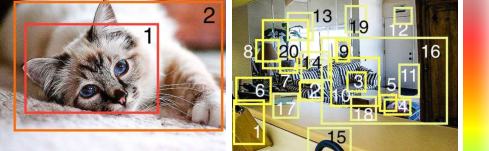
\includegraphics[width=1.0\linewidth]{introduction/intelligent_dialogs.pdf}
  \caption{Two different cases for verifying annotations in an image \cite{Konyushkova2017}. In the first case, with two high confidence predictions, a question asking interface is used. In the second case with many low confidence predictions, the user is asked to draw boxes from scratch. }
  \label{fig:intelligent_dialogs}
\end{figure}

Different kinds of annotation task can be approached in different ways, and in the case of verification based annotation the best option for having a user verify annotations might not be the same for every image. The focus of \cite{Konyushkova2017} is to intelligently chose the appropriate interface for the given image, and the quantity and type of prediction provided by a model. An example given is two images, one with two high scoring predictions, another with many low scoring predictions. To the first they have a user  verify each prediction by answering questions, to the first the user manually annotates boxes from scratch. At different points in the annotation process, the strength and accuracy of the model means that a different interface might be preferable even for the same image. When annotating data containing a commonly used object type (for example people, or cars), strong pretrained models exist. Starting from scratch on an difficult 

This work also tackles the same issue indirectly (in chapter \ref{chap:annotation}). The interface aims to cope with various situations by providing fine control over which object detections are displayed and allowing the user the most flexibility to decide which action to take. In the situation where a user is best to annotate boxes from scratch, the user can make that decision by clearing the existing boxes with a single click. In another situation many low confidence detections can be dealt with by using a high threshold, then allowing the user to view and verify low confidence detections by holding down a key. These approaches may not work in all situations, but seems to provide a useful trade off in many situations.









